\chapter{Flows validation plots}

\def\baseTag{_deta_uo}


\subsection{Tables}
\label{subapp:tables}


% It might be fun to see if the norm is better for the flow before the Xwt cut - but the reweighting isn't meaningful here
%\begin{table}
\centering
\caption{Yields for the predictions after applying the $X_{Wt}$ cut}
\label{tab:ks_Xwt_cut}
\begin{tabular}{lccc}
\toprule
{} &      obs &       rw &     flow \\
\midrule
3b1f        & 180044.0 & 175817.9 & 175416.8 \\
rev deta    &  16113.0 &  16462.7 &  16185.9 \\
lower left  &  40578.0 &  48708.9 &  39252.2 \\
lower right &  12377.0 &  14648.5 &  11982.7 \\
upper right &   5751.0 &   5543.0 &   5825.9 \\
upper left  &  19075.0 &  19504.7 &  19833.4 \\
4b SR       &  16171.0 &  15423.7 &  16564.8 \\
\bottomrule
\end{tabular}
\end{table}

%\begin{table}
\centering
\caption{Normalization differences for the predictions and the observed yields after applying the $X_{Wt}$ cut}
\label{tab:ks_Xwt_cut}
\begin{tabular}{lccc}
\toprule
{} &  1 - rw / obs [\%] &  1 - flow / obs [\%] \\
\midrule
3b1f        &                2.3 &                  2.4 \\
rev deta    &               -2.2 &                 -1.1 \\
lower left  &                -20 &                    3 \\
lower right &                -18 &                  3.3 \\
upper right &                3.6 &                 -3.2 \\
upper left  &               -2.3 &                 -5.7 \\
4b SR       &                4.6 &                 -2.7 \\
\bottomrule
\end{tabular}
\end{table}

%
%
%\begin{table}
\centering
\caption{Yields for the predictions before applying the $X_{Wt}$ cut}
\label{tab:ks}
\begin{tabular}{lccc}
\toprule
{} &      obs &       rw &     flow \\
\midrule
3b1f        & 224960.0 & 216283.6 & 218526.0 \\
rev deta    &  20440.0 &  19592.2 &  20619.6 \\
lower left  &  68908.0 &  66864.8 &  66781.1 \\
lower right &  16021.0 &  16782.4 &  15586.0 \\
upper right &   6492.0 &   5944.7 &   6622.7 \\
upper left  &  30508.0 &  28103.9 &  32603.3 \\
4b SR       &  21890.0 &  19350.8 &  21814.1 \\
\bottomrule
\end{tabular}
\end{table}

%\begin{table}
\centering
\caption{Normalization differences for the predictions and the observed yields before applying the $X_{Wt}$ cut}
\label{tab:ks}
\begin{tabular}{lccc}
\toprule
{} &  1 - rw / obs [\%] &  1 - flow / obs [\%] \\
\midrule
3b1f        &                3.9 &                  2.9 \\
rev deta    &                4.1 &                -0.88 \\
lower left  &                  3 &                  3.1 \\
lower right &               -4.8 &                  2.7 \\
upper right &                8.4 &                   -2 \\
upper left  &                7.9 &                 -6.9 \\
4b SR       &                 12 &                 0.35 \\
\bottomrule
\end{tabular}
\end{table}


% Honestly - I don't think these tables tell me a whole lot
%\foreach \tag in {_Xwt_cut, }{
%	\foreach \metric in {chi2_ndf, kl, ks} {
%		\small{\input{figures/flows/tables/\metric\tag}}
%		
%	}
%}

\begin{table}
\centering
\caption{Fitted length scales from the GP fit.}
\label{tab:len-scales}
\begin{tabular}{lcccccc}
\toprule
{} & \multicolumn{2}{c}{2016} & \multicolumn{2}{c}{2017} & \multicolumn{2}{c}{2018} \\
{} & $m_{H1}$ & $m_{H2}$ & $m_{H1}$ & $m_{H2}$ & $m_{H1}$ & $m_{H2}$ \\
\midrule
3b1f        &    101.9 &    51.31 &    94.13 &    64.32 &    100.1 &    50.17 \\
rev deta    &    59.76 &    64.87 &    63.62 &    68.51 &    60.68 &    68.57 \\
lower left  &    17.28 &    18.46 &    17.28 &    18.74 &    17.28 &    18.15 \\
lower right &     19.7 &    72.56 &    18.83 &    69.19 &    18.82 &    68.08 \\
upper right &    77.97 &    40.43 &    86.04 &    54.22 &    79.21 &    38.76 \\
upper left  &    91.43 &    24.69 &    85.82 &    24.95 &    88.94 &    23.08 \\
4b SR       &    108.3 &    50.62 &    106.1 &    64.38 &    105.4 &    56.38 \\
\bottomrule
\end{tabular}
\end{table}

\begin{table}
\centering
\caption{Fitted length scales from the GP fit.}
\label{tab:len-scales}
\begin{tabular}{lcccccc}
\toprule
{} &   2016 &   2017 &   2018 \\
\midrule
3b1f        &  81.85 &  54.76 &  178.2 \\
rev deta    & -297.8 & -285.3 & -191.6 \\
lower left  & -189.5 & -152.5 & -87.67 \\
lower right & -310.9 & -274.9 & -191.8 \\
upper right & -386.5 & -354.7 & -252.5 \\
upper left  & -229.6 & -222.3 & -117.6 \\
4b SR       & -214.6 &   -176 & -94.59 \\
\bottomrule
\end{tabular}
\end{table}


\FloatBarrier
\clearpage
%%%%%%%%%%%%%%%%%%%%%%%%%%%%%%
% Reversed deta_hh
%%%%%%%%%%%%%%%%%%%%%%%%%%%%%%
\subsection{Reversed \texorpdfstring{ $\Delta \eta_{HH}$}{Lg}}
\label{subapp:rev_deta}

\def\valreg{rev_deta}
\def\vallabel{reversed $\Delta \eta_{HH}$}

\def\figpath{figures/flows/\valreg/}

% GP plots
\begin{figure}[hb]
    \centering
    \subfloat{ 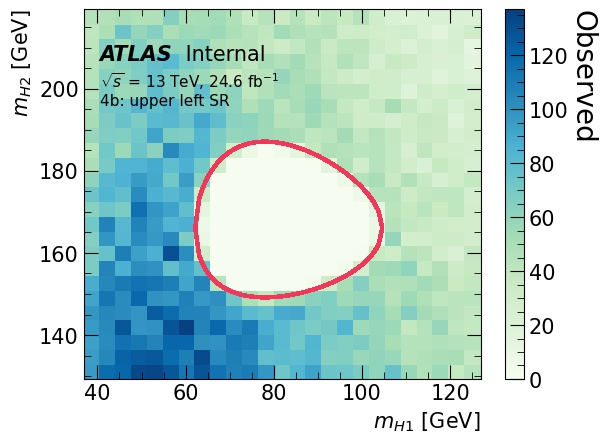
\includegraphics[width=0.22\textwidth]{\figpath/massplane_obs_16} }   
    \subfloat{ 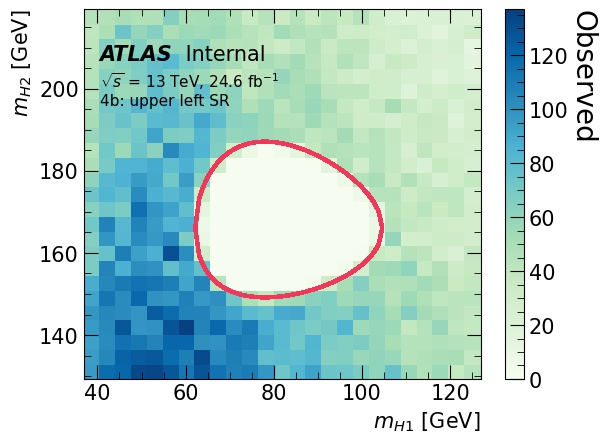
\includegraphics[width=0.22\textwidth]{\figpath/massplane_obs_16} }   
    \subfloat{ 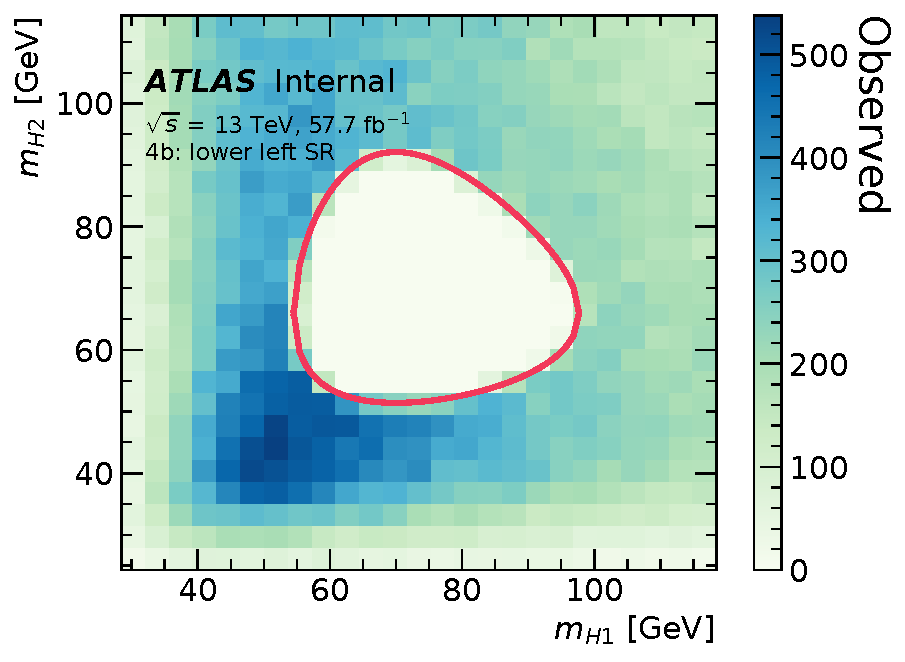
\includegraphics[width=0.22\textwidth]{\figpath/massplane_obs_18} }   
    \\
    \subfloat {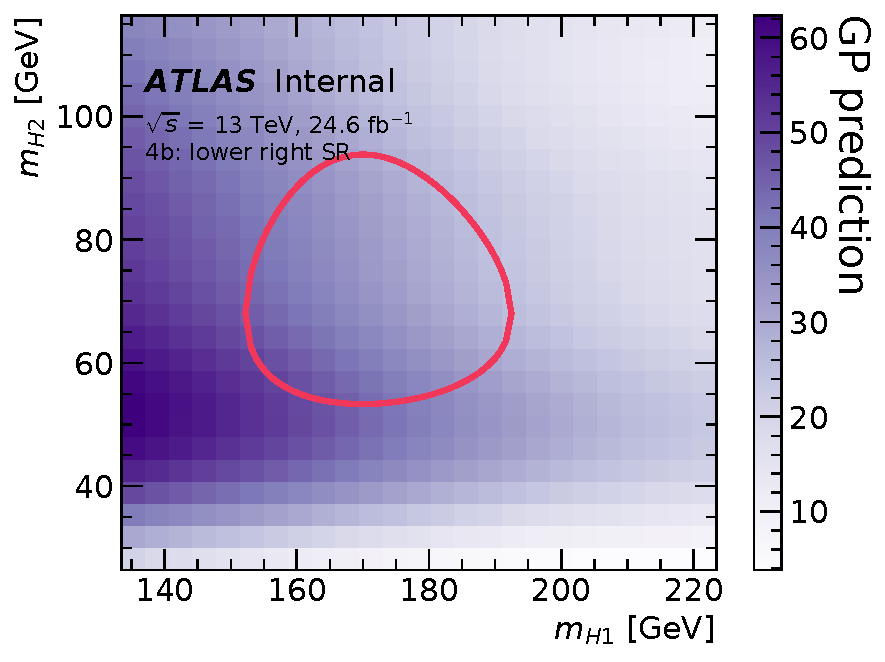
\includegraphics[width=0.22\textwidth]{\figpath/massplane_pred_16} }   
    \subfloat{ 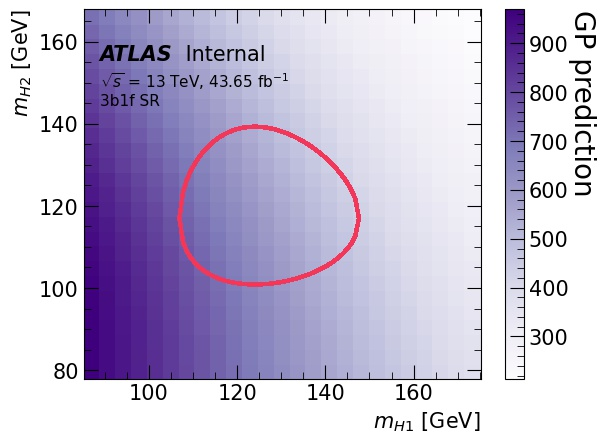
\includegraphics[width=0.22\textwidth]{\figpath/massplane_pred_17} }   
    \subfloat{ 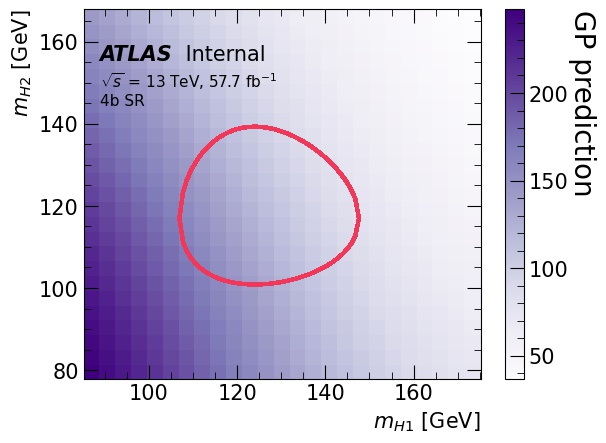
\includegraphics[width=0.22\textwidth]{\figpath/massplane_pred_18} }   
    \\
    \subfloat{ 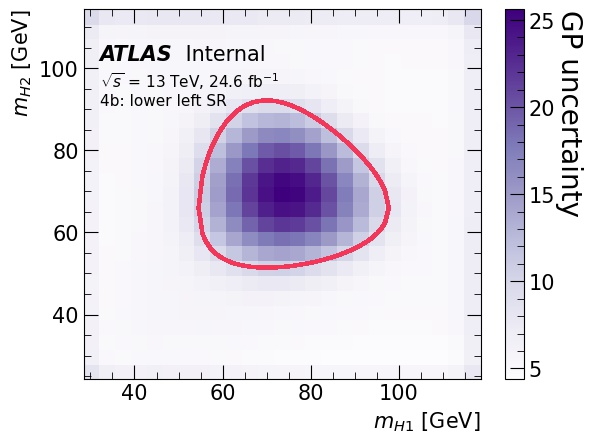
\includegraphics[width=0.22\textwidth]{\figpath/massplane_prederr_16} }   
    \subfloat{ 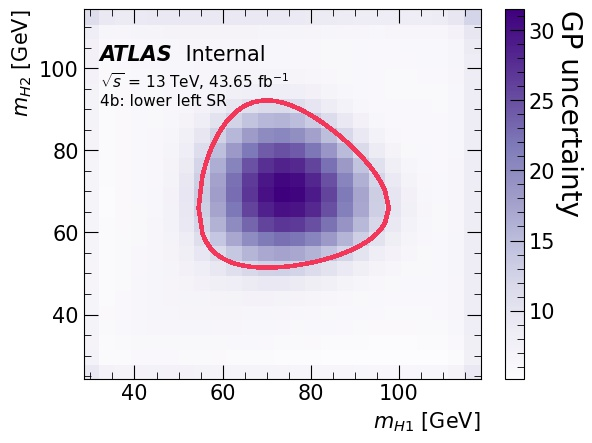
\includegraphics[width=0.22\textwidth]{\figpath/massplane_prederr_17} }   
    \subfloat{ 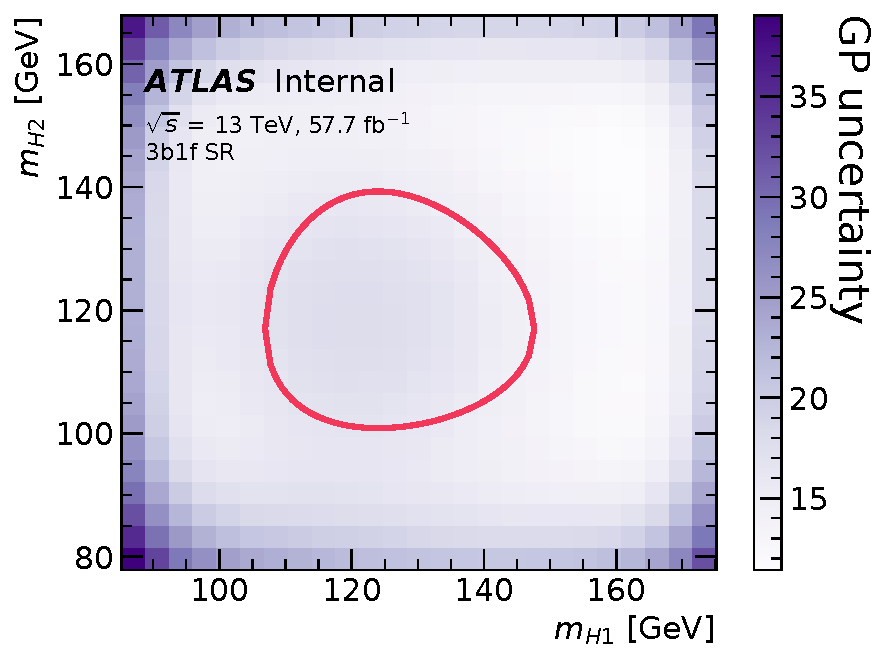
\includegraphics[width=0.22\textwidth]{\figpath/massplane_prederr_18} }   
    \\
    \subfloat{ 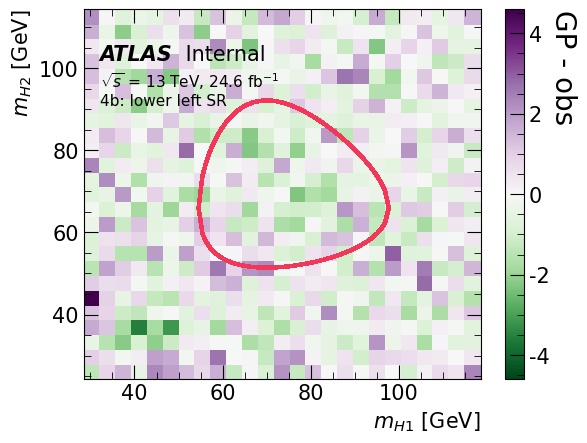
\includegraphics[width=0.22\textwidth]{\figpath/massplane_pred_minus_obs_over_sqrt_obs_16} }
    \subfloat{ 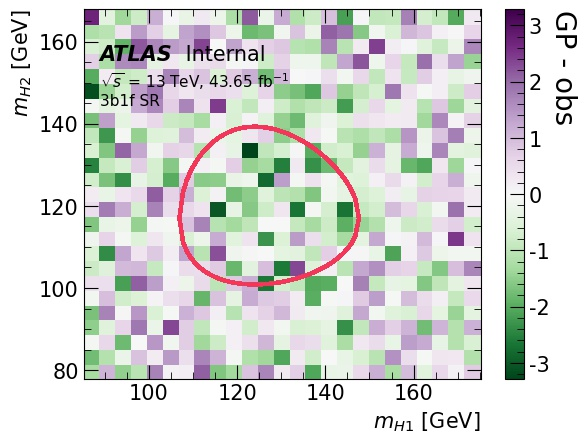
\includegraphics[width=0.22\textwidth]{\figpath/massplane_pred_minus_obs_over_sqrt_obs_17} }
    \subfloat{ 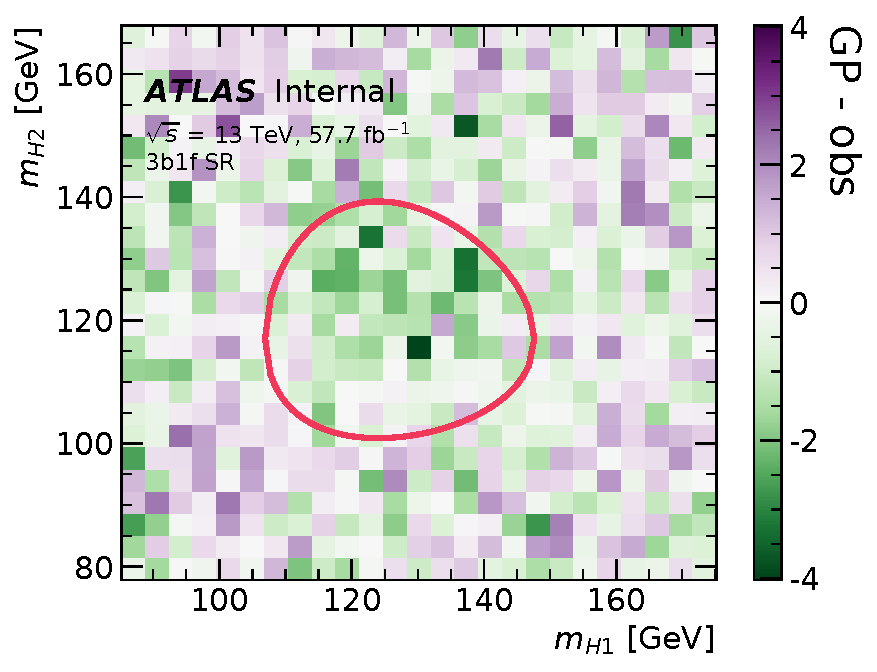
\includegraphics[width=0.22\textwidth]{\figpath/massplane_pred_minus_obs_over_sqrt_obs_18} }
    \\
    \subfloat{ 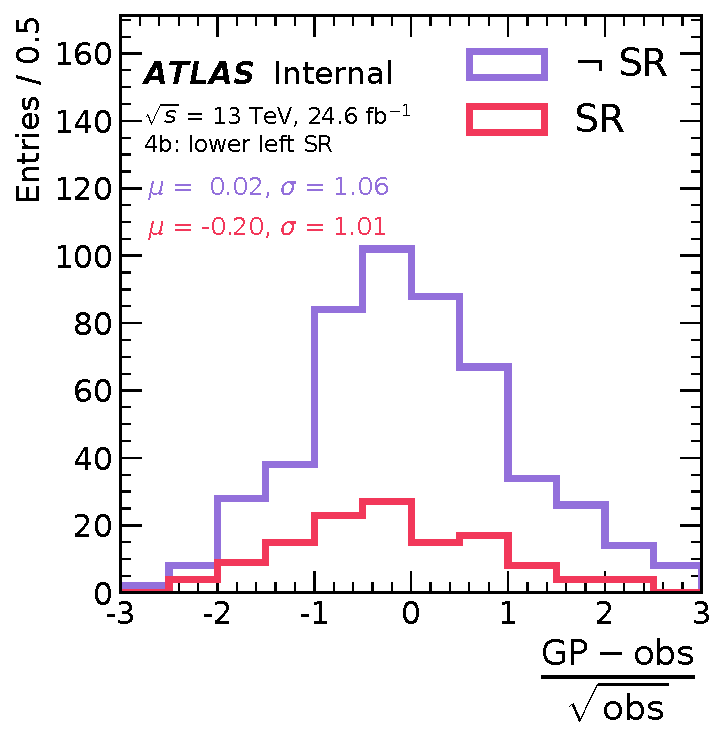
\includegraphics[width=0.18\textwidth]{\figpath/hist_pred_minus_obs_over_sqrt_obs_16}} \qquad
    \subfloat{ 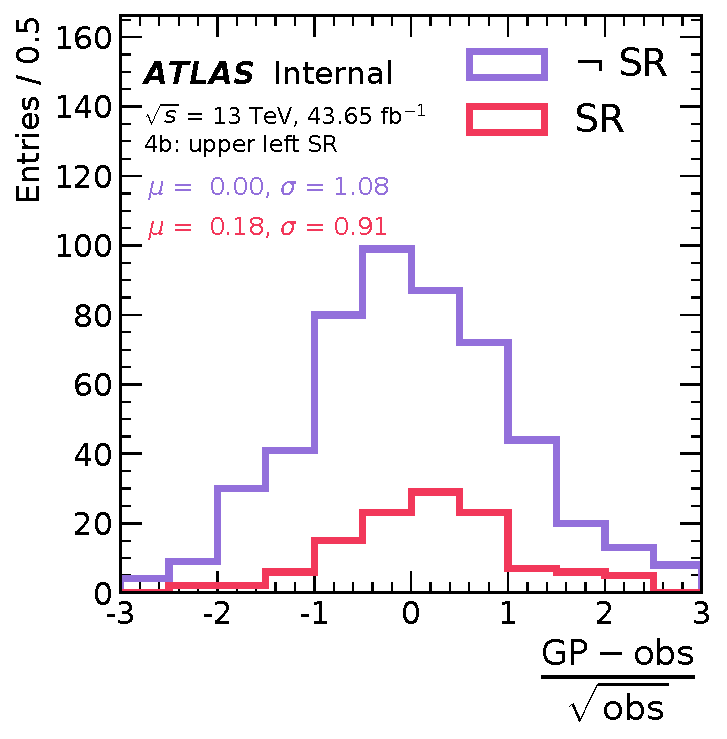
\includegraphics[width=0.18\textwidth]{\figpath/hist_pred_minus_obs_over_sqrt_obs_17}} \qquad
    \subfloat{ 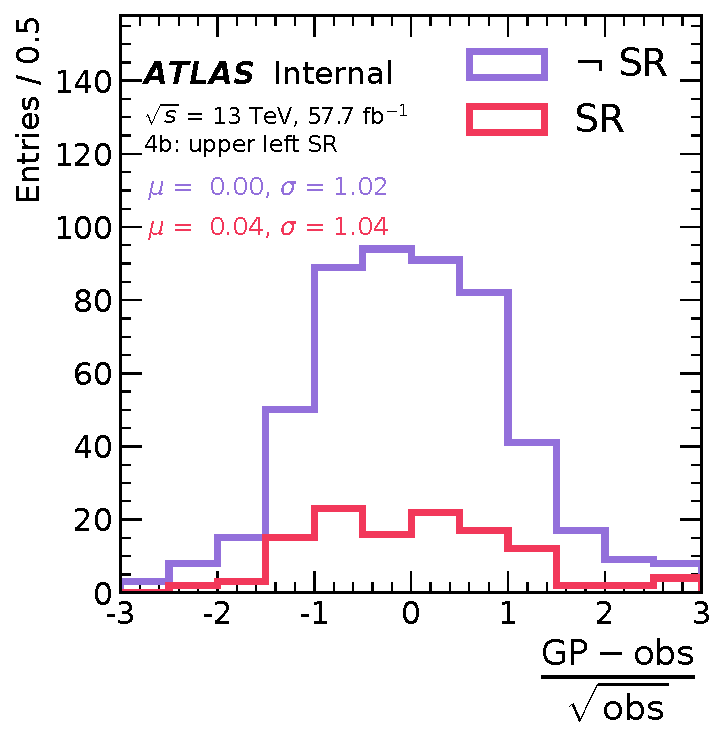
\includegraphics[width=0.18\textwidth]{\figpath/hist_pred_minus_obs_over_sqrt_obs_18}}
    \caption{GP fits for the \vallabel. All massplane fits are before the $X_{Wt}$ cut.}
    \label{fig:gp-\valreg}
\end{figure}

% The rest of the marginals
\begin{figure}[hbt]
    \centering
    \subfloat{ \includegraphics[width=0.3\textwidth]{\figpath/pT_h1_SR_Xwt_cut_rw_100_bs\baseTag.pdf} }
    \subfloat{ \includegraphics[width=0.3\textwidth]{\figpath/eta_h1_SR_Xwt_cut_rw_100_bs\baseTag.pdf} }
    \subfloat{ \includegraphics[width=0.3\textwidth]{\figpath/dphi_hh_SR_Xwt_cut_rw_100_bs\baseTag.pdf} }
    \\
    \subfloat{ \includegraphics[width=0.3\textwidth]{\figpath/pT_h2_SR_Xwt_cut_rw_100_bs\baseTag.pdf} }
    \subfloat{ \includegraphics[width=0.3\textwidth]{\figpath/eta_h2_SR_Xwt_cut_rw_100_bs\baseTag.pdf} }
    \subfloat{ \includegraphics[width=0.3\textwidth]{\figpath/X_wt_tag_SR_Xwt_cut_rw_100_bs\baseTag.pdf} }
    \\
    \subfloat{ \includegraphics[width=0.3\textwidth]{\figpath/m_hh_SR_Xwt_cut_rw_100_bs\baseTag.pdf} }
    \subfloat{ \includegraphics[width=0.3\textwidth]{\figpath/m_hh_cor2_SR_Xwt_cut_rw_100_bs\baseTag.pdf} }
    \subfloat{ \includegraphics[width=0.3\textwidth]{\figpath/dEta_hh_SR_Xwt_cut_rw_100_bs\baseTag.pdf} }
    \caption{Training and high level variables (post the $X_{Wt}$ cut) in the \vallabel validation region.}
    \label{fig:trainingvars-\valreg}
\end{figure}

\begin{figure}[hbt]
    \centering
    \subfloat{ \includegraphics[width=0.3\textwidth]{\figpath/pT_h1_SR_flow\baseTag.pdf} } 
    \subfloat{ \includegraphics[width=0.3\textwidth]{\figpath/eta_h1_SR_flow\baseTag.pdf} } 
    \subfloat{ \includegraphics[width=0.3\textwidth]{\figpath/dphi_hh_SR_flow\baseTag.pdf} } 
    \\
    \subfloat{ \includegraphics[width=0.3\textwidth]{\figpath/pT_h2_SR_flow\baseTag.pdf} }
    \subfloat{ \includegraphics[width=0.3\textwidth]{\figpath/eta_h2_SR_flow\baseTag.pdf} }
    \subfloat{ \includegraphics[width=0.3\textwidth]{\figpath/X_wt_tag_SR_flow\baseTag.pdf} }
    \\
    \subfloat{ \includegraphics[width=0.3\textwidth]{\figpath/m_hh_SR_flow\baseTag.pdf} }
    %\subfloat{ 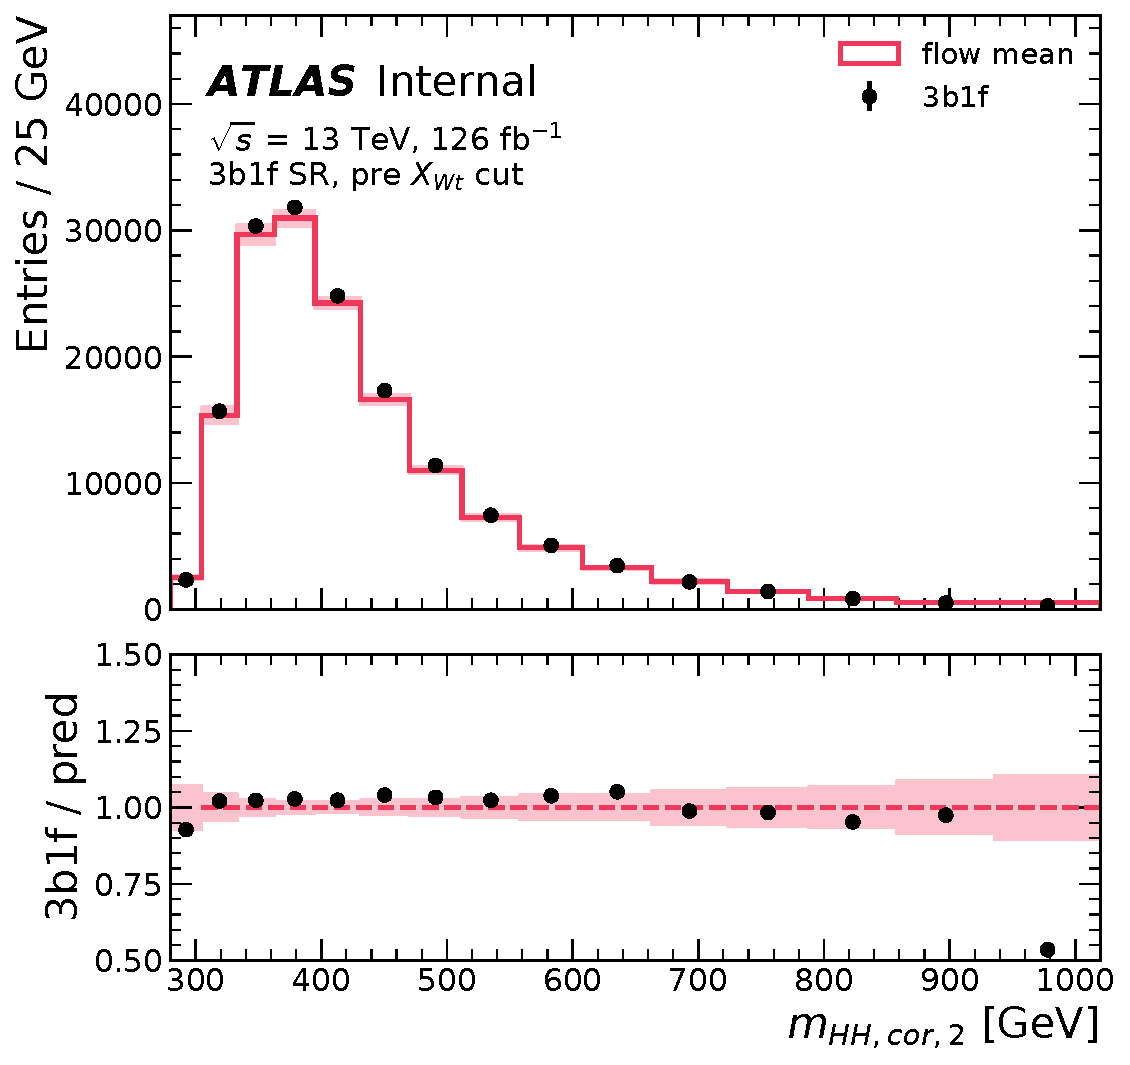
\includegraphics[width=0.3\textwidth]{\figpath/m_hh_cor2_SR_flow.pdf} }
    \subfloat{ \includegraphics[width=0.3\textwidth]{\figpath/dEta_hh_SR_flow\baseTag.pdf} }
    \subfloat{ \includegraphics[width=0.3\textwidth]{\figpath/pt_hh_SR_flow\baseTag.pdf} }
    \caption{Training variables (before applying the $X_{Wt}$ cut) in the \vallabel validation region.} 
    \label{fig:trainingvars-pre-Xwt-\valreg}
\end{figure}



% The high level discriminant plots
\begin{figure}[hbt]
    \centering
    \subfloat[After the $X_{Wt}$ cut]{ \includegraphics[width=\textwidth]{\figpath/X_hh_dEta_hh_m_hh_SR_Xwt_cut_rw_100_bs\baseTag.pdf} } \\
    \subfloat[Before the $X_{Wt}$ cut]{ \includegraphics[width=\textwidth]{\figpath/X_hh_dEta_hh_m_hh_SR_flow\baseTag.pdf} }
    \caption{High dimensional discriminant in the \vallabel validation region.}
    \label{fig:ggF-discs-\valreg}
\end{figure}

\FloatBarrier

%%%%%%%%%%%%%%%%%%%%%%%%%%%%%%
% Shifted regions
%%%%%%%%%%%%%%%%%%%%%%%%%%%%%%
\subsection{Shifted regions}
\label{subapp:shifted-regs}

\def\valreg{LL}
\def\vallabel{lower left SR}

\def\figpath{figures/flows/\valreg/}

% GP plots
\begin{figure}[hb]
    \centering
    \subfloat{ 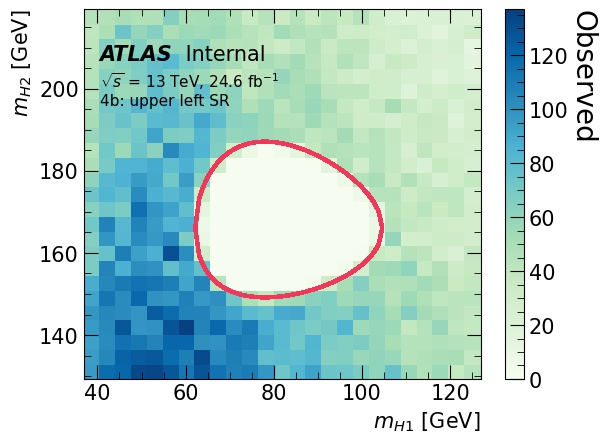
\includegraphics[width=0.22\textwidth]{\figpath/massplane_obs_16} }   
    \subfloat{ 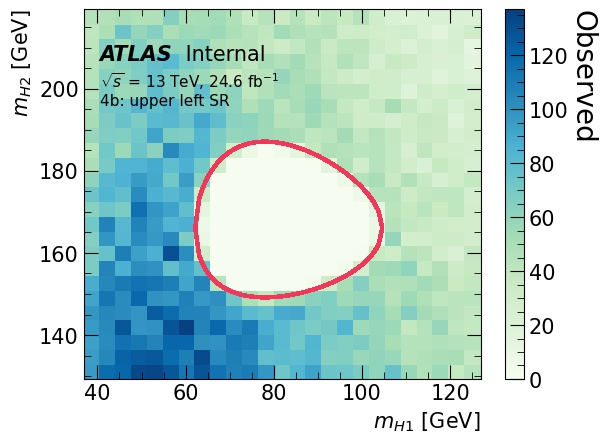
\includegraphics[width=0.22\textwidth]{\figpath/massplane_obs_16} }   
    \subfloat{ 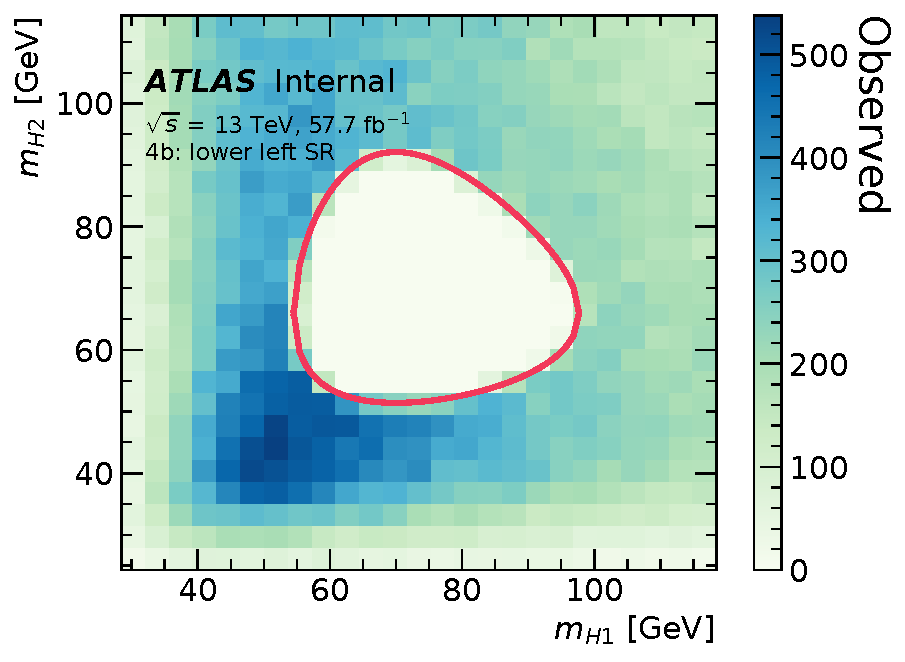
\includegraphics[width=0.22\textwidth]{\figpath/massplane_obs_18} }   
    \\
    \subfloat {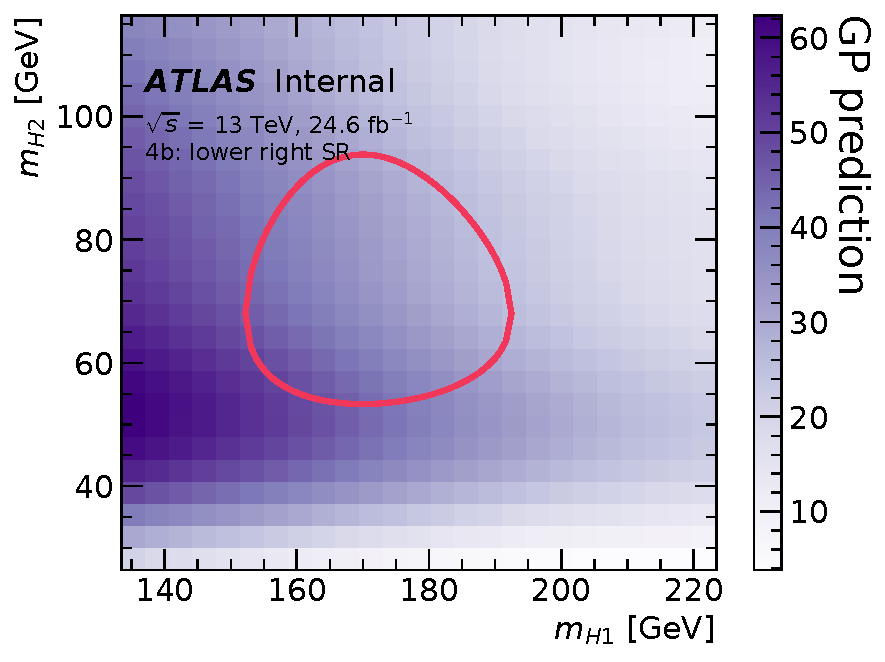
\includegraphics[width=0.22\textwidth]{\figpath/massplane_pred_16} }   
    \subfloat{ 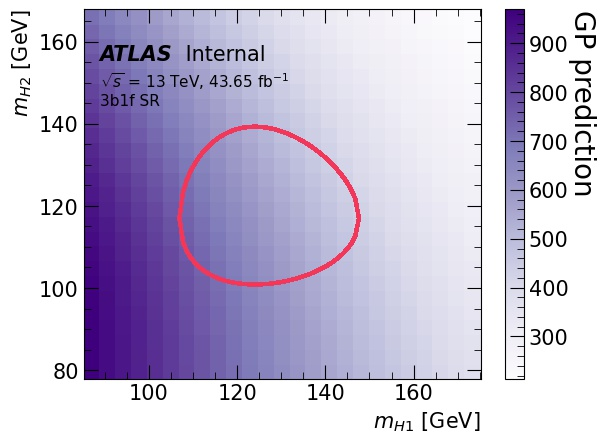
\includegraphics[width=0.22\textwidth]{\figpath/massplane_pred_17} }   
    \subfloat{ 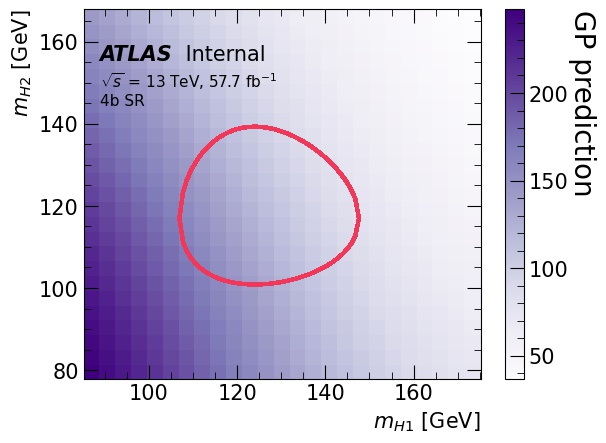
\includegraphics[width=0.22\textwidth]{\figpath/massplane_pred_18} }   
    \\
    \subfloat{ 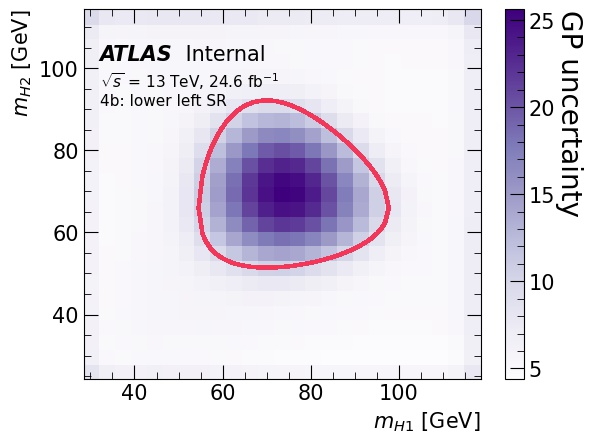
\includegraphics[width=0.22\textwidth]{\figpath/massplane_prederr_16} }   
    \subfloat{ 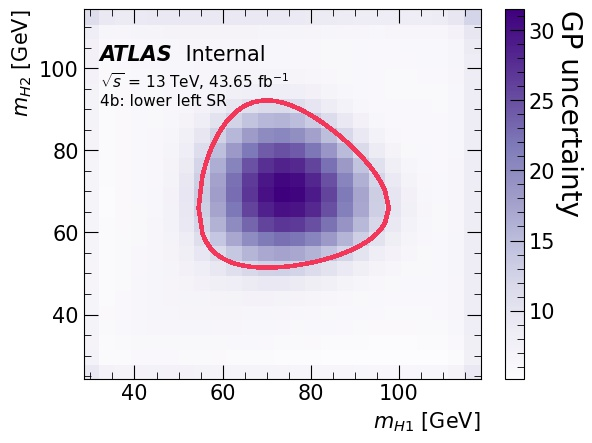
\includegraphics[width=0.22\textwidth]{\figpath/massplane_prederr_17} }   
    \subfloat{ 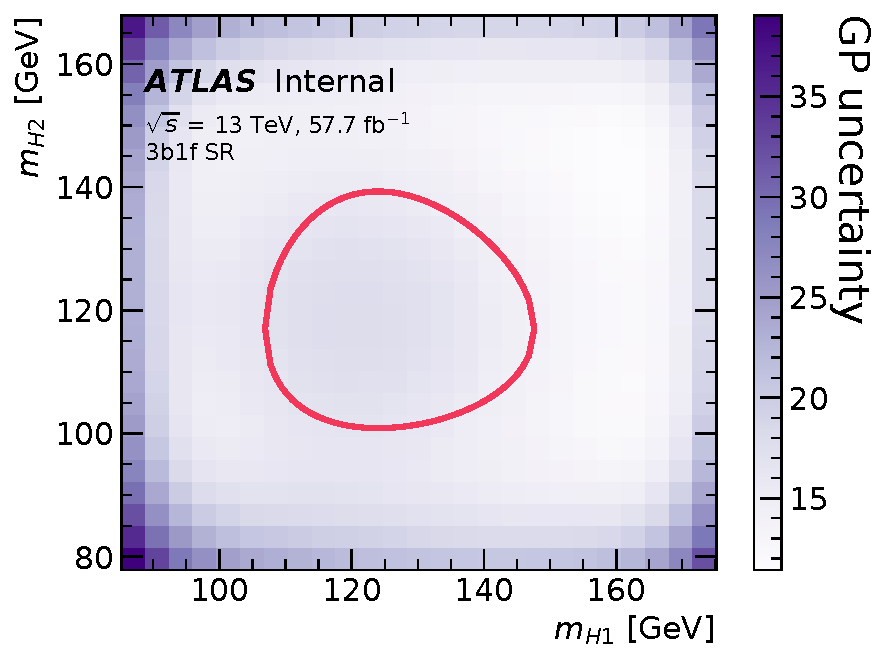
\includegraphics[width=0.22\textwidth]{\figpath/massplane_prederr_18} }   
    \\
    \subfloat{ 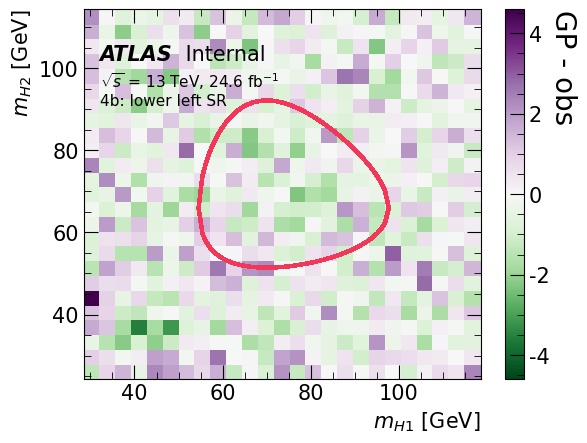
\includegraphics[width=0.22\textwidth]{\figpath/massplane_pred_minus_obs_over_sqrt_obs_16} }
    \subfloat{ 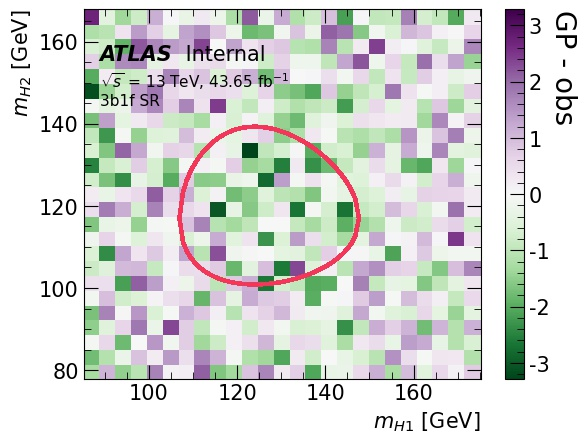
\includegraphics[width=0.22\textwidth]{\figpath/massplane_pred_minus_obs_over_sqrt_obs_17} }
    \subfloat{ 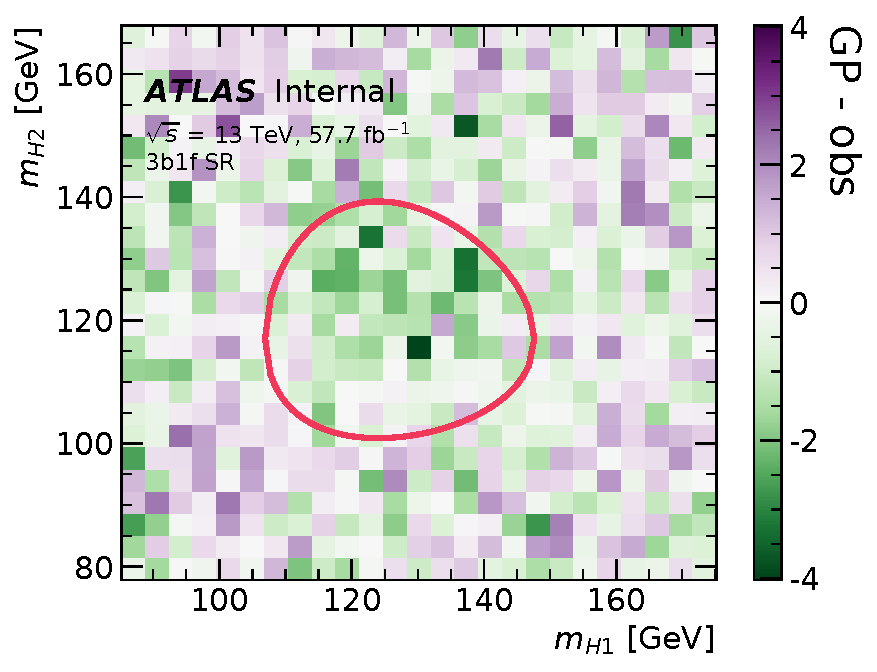
\includegraphics[width=0.22\textwidth]{\figpath/massplane_pred_minus_obs_over_sqrt_obs_18} }
    \\
    \subfloat{ 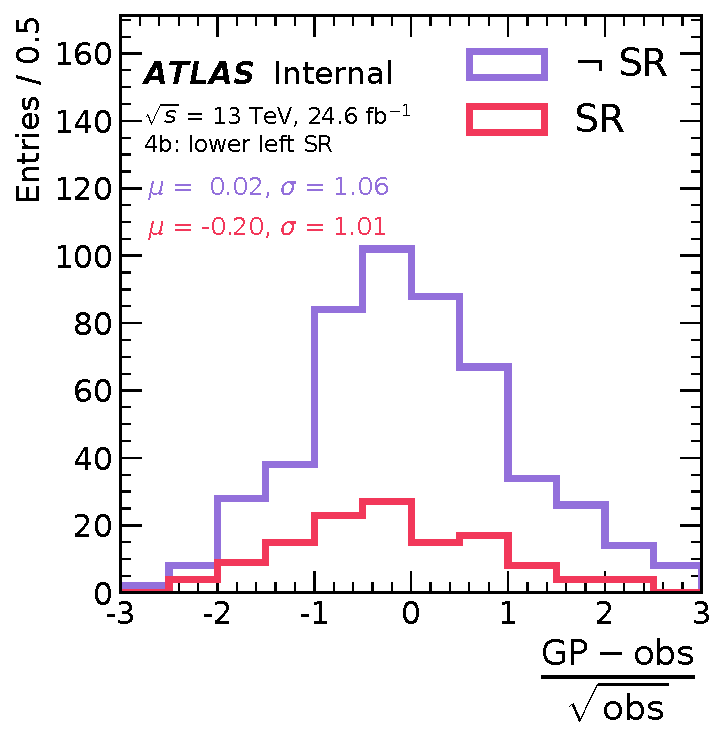
\includegraphics[width=0.18\textwidth]{\figpath/hist_pred_minus_obs_over_sqrt_obs_16}} \qquad
    \subfloat{ 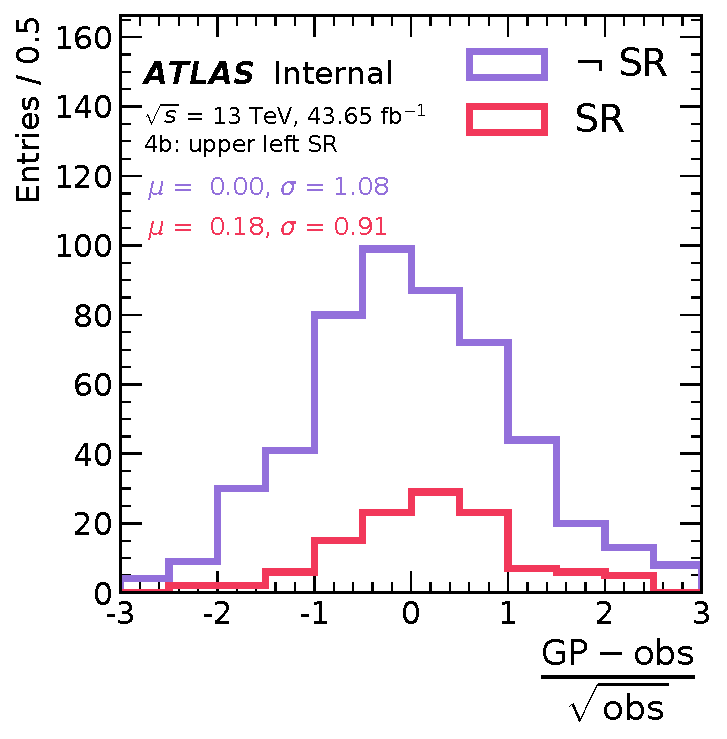
\includegraphics[width=0.18\textwidth]{\figpath/hist_pred_minus_obs_over_sqrt_obs_17}} \qquad
    \subfloat{ \includegraphics[width=0.18\textwidth]{\figpath/hist_pred_minus_obs_over_sqrt_obs_18}}
    \caption{GP fits for the \vallabel. All massplane fits are before the $X_{Wt}$ cut.}
    \label{fig:gp-\valreg}
\end{figure}

% The rest of the marginals
\begin{figure}[hbt]
    \centering
    \subfloat{ \includegraphics[width=0.3\textwidth]{\figpath/pT_h1_SR_Xwt_cut_rw_100_bs\baseTag.pdf} }
    \subfloat{ \includegraphics[width=0.3\textwidth]{\figpath/eta_h1_SR_Xwt_cut_rw_100_bs\baseTag.pdf} }
    \subfloat{ \includegraphics[width=0.3\textwidth]{\figpath/dphi_hh_SR_Xwt_cut_rw_100_bs\baseTag.pdf} }
    \\
    \subfloat{ \includegraphics[width=0.3\textwidth]{\figpath/pT_h2_SR_Xwt_cut_rw_100_bs\baseTag.pdf} }
    \subfloat{ \includegraphics[width=0.3\textwidth]{\figpath/eta_h2_SR_Xwt_cut_rw_100_bs\baseTag.pdf} }
    \subfloat{ \includegraphics[width=0.3\textwidth]{\figpath/X_wt_tag_SR_Xwt_cut_rw_100_bs\baseTag.pdf} }
    \\
    \subfloat{ \includegraphics[width=0.3\textwidth]{\figpath/m_hh_SR_Xwt_cut_rw_100_bs\baseTag.pdf} }
    \subfloat{ \includegraphics[width=0.3\textwidth]{\figpath/m_hh_cor2_SR_Xwt_cut_rw_100_bs\baseTag.pdf} }
    \subfloat{ \includegraphics[width=0.3\textwidth]{\figpath/dEta_hh_SR_Xwt_cut_rw_100_bs\baseTag.pdf} }
    \caption{Training and high level variables (post the $X_{Wt}$ cut) in the \vallabel validation region.}
    \label{fig:trainingvars-\valreg}
\end{figure}

\begin{figure}[hbt]
    \centering
    \subfloat{ \includegraphics[width=0.3\textwidth]{\figpath/pT_h1_SR_flow\baseTag.pdf} } 
    \subfloat{ \includegraphics[width=0.3\textwidth]{\figpath/eta_h1_SR_flow\baseTag.pdf} } 
    \subfloat{ \includegraphics[width=0.3\textwidth]{\figpath/dphi_hh_SR_flow\baseTag.pdf} } 
    \\
    \subfloat{ \includegraphics[width=0.3\textwidth]{\figpath/pT_h2_SR_flow\baseTag.pdf} }
    \subfloat{ \includegraphics[width=0.3\textwidth]{\figpath/eta_h2_SR_flow\baseTag.pdf} }
    \subfloat{ \includegraphics[width=0.3\textwidth]{\figpath/X_wt_tag_SR_flow\baseTag.pdf} }
    \\
    \subfloat{ \includegraphics[width=0.3\textwidth]{\figpath/m_hh_SR_flow\baseTag.pdf} }
    %\subfloat{ \includegraphics[width=0.3\textwidth]{\figpath/m_hh_cor2_SR_flow.pdf} }
    \subfloat{ \includegraphics[width=0.3\textwidth]{\figpath/dEta_hh_SR_flow\baseTag.pdf} }
    \subfloat{ \includegraphics[width=0.3\textwidth]{\figpath/pt_hh_SR_flow\baseTag.pdf} }
    \caption{Training variables (before applying the $X_{Wt}$ cut) in the \vallabel validation region.} 
    \label{fig:trainingvars-pre-Xwt-\valreg}
\end{figure}



% The high level discriminant plots
\begin{figure}[hbt]
    \centering
    \subfloat[After the $X_{Wt}$ cut]{ \includegraphics[width=\textwidth]{\figpath/X_hh_dEta_hh_m_hh_SR_Xwt_cut_rw_100_bs\baseTag.pdf} } \\
    \subfloat[Before the $X_{Wt}$ cut]{ \includegraphics[width=\textwidth]{\figpath/X_hh_dEta_hh_m_hh_SR_flow\baseTag.pdf} }
    \caption{High dimensional discriminant in the \vallabel validation region.}
    \label{fig:ggF-discs-\valreg}
\end{figure}

\FloatBarrier


\def\valreg{LR}
\def\vallabel{lower right SR}

\def\figpath{figures/flows/\valreg/}

% GP plots
\begin{figure}[hb]
    \centering
    \subfloat{ \includegraphics[width=0.22\textwidth]{\figpath/massplane_obs_16} }   
    \subfloat{ \includegraphics[width=0.22\textwidth]{\figpath/massplane_obs_16} }   
    \subfloat{ \includegraphics[width=0.22\textwidth]{\figpath/massplane_obs_18} }   
    \\
    \subfloat {\includegraphics[width=0.22\textwidth]{\figpath/massplane_pred_16} }   
    \subfloat{ \includegraphics[width=0.22\textwidth]{\figpath/massplane_pred_17} }   
    \subfloat{ \includegraphics[width=0.22\textwidth]{\figpath/massplane_pred_18} }   
    \\
    \subfloat{ \includegraphics[width=0.22\textwidth]{\figpath/massplane_prederr_16} }   
    \subfloat{ \includegraphics[width=0.22\textwidth]{\figpath/massplane_prederr_17} }   
    \subfloat{ \includegraphics[width=0.22\textwidth]{\figpath/massplane_prederr_18} }   
    \\
    \subfloat{ \includegraphics[width=0.22\textwidth]{\figpath/massplane_pred_minus_obs_over_sqrt_obs_16} }
    \subfloat{ \includegraphics[width=0.22\textwidth]{\figpath/massplane_pred_minus_obs_over_sqrt_obs_17} }
    \subfloat{ \includegraphics[width=0.22\textwidth]{\figpath/massplane_pred_minus_obs_over_sqrt_obs_18} }
    \\
    \subfloat{ \includegraphics[width=0.18\textwidth]{\figpath/hist_pred_minus_obs_over_sqrt_obs_16}} \qquad
    \subfloat{ \includegraphics[width=0.18\textwidth]{\figpath/hist_pred_minus_obs_over_sqrt_obs_17}} \qquad
    \subfloat{ \includegraphics[width=0.18\textwidth]{\figpath/hist_pred_minus_obs_over_sqrt_obs_18}}
    \caption{GP fits for the \vallabel. All massplane fits are before the $X_{Wt}$ cut.}
    \label{fig:gp-\valreg}
\end{figure}

% The rest of the marginals
\begin{figure}[hbt]
    \centering
    \subfloat{ \includegraphics[width=0.3\textwidth]{\figpath/pT_h1_SR_Xwt_cut_rw_100_bs\baseTag.pdf} }
    \subfloat{ \includegraphics[width=0.3\textwidth]{\figpath/eta_h1_SR_Xwt_cut_rw_100_bs\baseTag.pdf} }
    \subfloat{ \includegraphics[width=0.3\textwidth]{\figpath/dphi_hh_SR_Xwt_cut_rw_100_bs\baseTag.pdf} }
    \\
    \subfloat{ \includegraphics[width=0.3\textwidth]{\figpath/pT_h2_SR_Xwt_cut_rw_100_bs\baseTag.pdf} }
    \subfloat{ \includegraphics[width=0.3\textwidth]{\figpath/eta_h2_SR_Xwt_cut_rw_100_bs\baseTag.pdf} }
    \subfloat{ \includegraphics[width=0.3\textwidth]{\figpath/X_wt_tag_SR_Xwt_cut_rw_100_bs\baseTag.pdf} }
    \\
    \subfloat{ \includegraphics[width=0.3\textwidth]{\figpath/m_hh_SR_Xwt_cut_rw_100_bs\baseTag.pdf} }
    \subfloat{ \includegraphics[width=0.3\textwidth]{\figpath/m_hh_cor2_SR_Xwt_cut_rw_100_bs\baseTag.pdf} }
    \subfloat{ \includegraphics[width=0.3\textwidth]{\figpath/dEta_hh_SR_Xwt_cut_rw_100_bs\baseTag.pdf} }
    \caption{Training and high level variables (post the $X_{Wt}$ cut) in the \vallabel validation region.}
    \label{fig:trainingvars-\valreg}
\end{figure}

\begin{figure}[hbt]
    \centering
    \subfloat{ \includegraphics[width=0.3\textwidth]{\figpath/pT_h1_SR_flow\baseTag.pdf} } 
    \subfloat{ \includegraphics[width=0.3\textwidth]{\figpath/eta_h1_SR_flow\baseTag.pdf} } 
    \subfloat{ \includegraphics[width=0.3\textwidth]{\figpath/dphi_hh_SR_flow\baseTag.pdf} } 
    \\
    \subfloat{ \includegraphics[width=0.3\textwidth]{\figpath/pT_h2_SR_flow\baseTag.pdf} }
    \subfloat{ \includegraphics[width=0.3\textwidth]{\figpath/eta_h2_SR_flow\baseTag.pdf} }
    \subfloat{ \includegraphics[width=0.3\textwidth]{\figpath/X_wt_tag_SR_flow\baseTag.pdf} }
    \\
    \subfloat{ \includegraphics[width=0.3\textwidth]{\figpath/m_hh_SR_flow\baseTag.pdf} }
    %\subfloat{ \includegraphics[width=0.3\textwidth]{\figpath/m_hh_cor2_SR_flow.pdf} }
    \subfloat{ \includegraphics[width=0.3\textwidth]{\figpath/dEta_hh_SR_flow\baseTag.pdf} }
    \subfloat{ \includegraphics[width=0.3\textwidth]{\figpath/pt_hh_SR_flow\baseTag.pdf} }
    \caption{Training variables (before applying the $X_{Wt}$ cut) in the \vallabel validation region.} 
    \label{fig:trainingvars-pre-Xwt-\valreg}
\end{figure}



% The high level discriminant plots
\begin{figure}[hbt]
    \centering
    \subfloat[After the $X_{Wt}$ cut]{ \includegraphics[width=\textwidth]{\figpath/X_hh_dEta_hh_m_hh_SR_Xwt_cut_rw_100_bs\baseTag.pdf} } \\
    \subfloat[Before the $X_{Wt}$ cut]{ \includegraphics[width=\textwidth]{\figpath/X_hh_dEta_hh_m_hh_SR_flow\baseTag.pdf} }
    \caption{High dimensional discriminant in the \vallabel validation region.}
    \label{fig:ggF-discs-\valreg}
\end{figure}

\FloatBarrier


\def\valreg{UR}
\def\vallabel{upper right SR}

\def\figpath{figures/flows/\valreg/}

% GP plots
\begin{figure}[hb]
    \centering
    \subfloat{ \includegraphics[width=0.22\textwidth]{\figpath/massplane_obs_16} }   
    \subfloat{ \includegraphics[width=0.22\textwidth]{\figpath/massplane_obs_16} }   
    \subfloat{ \includegraphics[width=0.22\textwidth]{\figpath/massplane_obs_18} }   
    \\
    \subfloat {\includegraphics[width=0.22\textwidth]{\figpath/massplane_pred_16} }   
    \subfloat{ \includegraphics[width=0.22\textwidth]{\figpath/massplane_pred_17} }   
    \subfloat{ \includegraphics[width=0.22\textwidth]{\figpath/massplane_pred_18} }   
    \\
    \subfloat{ \includegraphics[width=0.22\textwidth]{\figpath/massplane_prederr_16} }   
    \subfloat{ \includegraphics[width=0.22\textwidth]{\figpath/massplane_prederr_17} }   
    \subfloat{ \includegraphics[width=0.22\textwidth]{\figpath/massplane_prederr_18} }   
    \\
    \subfloat{ \includegraphics[width=0.22\textwidth]{\figpath/massplane_pred_minus_obs_over_sqrt_obs_16} }
    \subfloat{ \includegraphics[width=0.22\textwidth]{\figpath/massplane_pred_minus_obs_over_sqrt_obs_17} }
    \subfloat{ \includegraphics[width=0.22\textwidth]{\figpath/massplane_pred_minus_obs_over_sqrt_obs_18} }
    \\
    \subfloat{ \includegraphics[width=0.18\textwidth]{\figpath/hist_pred_minus_obs_over_sqrt_obs_16}} \qquad
    \subfloat{ \includegraphics[width=0.18\textwidth]{\figpath/hist_pred_minus_obs_over_sqrt_obs_17}} \qquad
    \subfloat{ \includegraphics[width=0.18\textwidth]{\figpath/hist_pred_minus_obs_over_sqrt_obs_18}}
    \caption{GP fits for the \vallabel. All massplane fits are before the $X_{Wt}$ cut.}
    \label{fig:gp-\valreg}
\end{figure}

% The rest of the marginals
\begin{figure}[hbt]
    \centering
    \subfloat{ \includegraphics[width=0.3\textwidth]{\figpath/pT_h1_SR_Xwt_cut_rw_100_bs\baseTag.pdf} }
    \subfloat{ \includegraphics[width=0.3\textwidth]{\figpath/eta_h1_SR_Xwt_cut_rw_100_bs\baseTag.pdf} }
    \subfloat{ \includegraphics[width=0.3\textwidth]{\figpath/dphi_hh_SR_Xwt_cut_rw_100_bs\baseTag.pdf} }
    \\
    \subfloat{ \includegraphics[width=0.3\textwidth]{\figpath/pT_h2_SR_Xwt_cut_rw_100_bs\baseTag.pdf} }
    \subfloat{ \includegraphics[width=0.3\textwidth]{\figpath/eta_h2_SR_Xwt_cut_rw_100_bs\baseTag.pdf} }
    \subfloat{ \includegraphics[width=0.3\textwidth]{\figpath/X_wt_tag_SR_Xwt_cut_rw_100_bs\baseTag.pdf} }
    \\
    \subfloat{ \includegraphics[width=0.3\textwidth]{\figpath/m_hh_SR_Xwt_cut_rw_100_bs\baseTag.pdf} }
    \subfloat{ \includegraphics[width=0.3\textwidth]{\figpath/m_hh_cor2_SR_Xwt_cut_rw_100_bs\baseTag.pdf} }
    \subfloat{ \includegraphics[width=0.3\textwidth]{\figpath/dEta_hh_SR_Xwt_cut_rw_100_bs\baseTag.pdf} }
    \caption{Training and high level variables (post the $X_{Wt}$ cut) in the \vallabel validation region.}
    \label{fig:trainingvars-\valreg}
\end{figure}

\begin{figure}[hbt]
    \centering
    \subfloat{ \includegraphics[width=0.3\textwidth]{\figpath/pT_h1_SR_flow\baseTag.pdf} } 
    \subfloat{ \includegraphics[width=0.3\textwidth]{\figpath/eta_h1_SR_flow\baseTag.pdf} } 
    \subfloat{ \includegraphics[width=0.3\textwidth]{\figpath/dphi_hh_SR_flow\baseTag.pdf} } 
    \\
    \subfloat{ \includegraphics[width=0.3\textwidth]{\figpath/pT_h2_SR_flow\baseTag.pdf} }
    \subfloat{ \includegraphics[width=0.3\textwidth]{\figpath/eta_h2_SR_flow\baseTag.pdf} }
    \subfloat{ \includegraphics[width=0.3\textwidth]{\figpath/X_wt_tag_SR_flow\baseTag.pdf} }
    \\
    \subfloat{ \includegraphics[width=0.3\textwidth]{\figpath/m_hh_SR_flow\baseTag.pdf} }
    %\subfloat{ \includegraphics[width=0.3\textwidth]{\figpath/m_hh_cor2_SR_flow.pdf} }
    \subfloat{ \includegraphics[width=0.3\textwidth]{\figpath/dEta_hh_SR_flow\baseTag.pdf} }
    \subfloat{ \includegraphics[width=0.3\textwidth]{\figpath/pt_hh_SR_flow\baseTag.pdf} }
    \caption{Training variables (before applying the $X_{Wt}$ cut) in the \vallabel validation region.} 
    \label{fig:trainingvars-pre-Xwt-\valreg}
\end{figure}



% The high level discriminant plots
\begin{figure}[hbt]
    \centering
    \subfloat[After the $X_{Wt}$ cut]{ \includegraphics[width=\textwidth]{\figpath/X_hh_dEta_hh_m_hh_SR_Xwt_cut_rw_100_bs\baseTag.pdf} } \\
    \subfloat[Before the $X_{Wt}$ cut]{ \includegraphics[width=\textwidth]{\figpath/X_hh_dEta_hh_m_hh_SR_flow\baseTag.pdf} }
    \caption{High dimensional discriminant in the \vallabel validation region.}
    \label{fig:ggF-discs-\valreg}
\end{figure}

\FloatBarrier


\def\valreg{UL}
\def\vallabel{upper left SR}

\def\figpath{figures/flows/\valreg/}

% GP plots
\begin{figure}[hb]
    \centering
    \subfloat{ \includegraphics[width=0.22\textwidth]{\figpath/massplane_obs_16} }   
    \subfloat{ \includegraphics[width=0.22\textwidth]{\figpath/massplane_obs_16} }   
    \subfloat{ \includegraphics[width=0.22\textwidth]{\figpath/massplane_obs_18} }   
    \\
    \subfloat {\includegraphics[width=0.22\textwidth]{\figpath/massplane_pred_16} }   
    \subfloat{ \includegraphics[width=0.22\textwidth]{\figpath/massplane_pred_17} }   
    \subfloat{ \includegraphics[width=0.22\textwidth]{\figpath/massplane_pred_18} }   
    \\
    \subfloat{ \includegraphics[width=0.22\textwidth]{\figpath/massplane_prederr_16} }   
    \subfloat{ \includegraphics[width=0.22\textwidth]{\figpath/massplane_prederr_17} }   
    \subfloat{ \includegraphics[width=0.22\textwidth]{\figpath/massplane_prederr_18} }   
    \\
    \subfloat{ \includegraphics[width=0.22\textwidth]{\figpath/massplane_pred_minus_obs_over_sqrt_obs_16} }
    \subfloat{ \includegraphics[width=0.22\textwidth]{\figpath/massplane_pred_minus_obs_over_sqrt_obs_17} }
    \subfloat{ \includegraphics[width=0.22\textwidth]{\figpath/massplane_pred_minus_obs_over_sqrt_obs_18} }
    \\
    \subfloat{ \includegraphics[width=0.18\textwidth]{\figpath/hist_pred_minus_obs_over_sqrt_obs_16}} \qquad
    \subfloat{ \includegraphics[width=0.18\textwidth]{\figpath/hist_pred_minus_obs_over_sqrt_obs_17}} \qquad
    \subfloat{ \includegraphics[width=0.18\textwidth]{\figpath/hist_pred_minus_obs_over_sqrt_obs_18}}
    \caption{GP fits for the \vallabel. All massplane fits are before the $X_{Wt}$ cut.}
    \label{fig:gp-\valreg}
\end{figure}

% The rest of the marginals
\begin{figure}[hbt]
    \centering
    \subfloat{ \includegraphics[width=0.3\textwidth]{\figpath/pT_h1_SR_Xwt_cut_rw_100_bs\baseTag.pdf} }
    \subfloat{ \includegraphics[width=0.3\textwidth]{\figpath/eta_h1_SR_Xwt_cut_rw_100_bs\baseTag.pdf} }
    \subfloat{ \includegraphics[width=0.3\textwidth]{\figpath/dphi_hh_SR_Xwt_cut_rw_100_bs\baseTag.pdf} }
    \\
    \subfloat{ \includegraphics[width=0.3\textwidth]{\figpath/pT_h2_SR_Xwt_cut_rw_100_bs\baseTag.pdf} }
    \subfloat{ \includegraphics[width=0.3\textwidth]{\figpath/eta_h2_SR_Xwt_cut_rw_100_bs\baseTag.pdf} }
    \subfloat{ \includegraphics[width=0.3\textwidth]{\figpath/X_wt_tag_SR_Xwt_cut_rw_100_bs\baseTag.pdf} }
    \\
    \subfloat{ \includegraphics[width=0.3\textwidth]{\figpath/m_hh_SR_Xwt_cut_rw_100_bs\baseTag.pdf} }
    \subfloat{ \includegraphics[width=0.3\textwidth]{\figpath/m_hh_cor2_SR_Xwt_cut_rw_100_bs\baseTag.pdf} }
    \subfloat{ \includegraphics[width=0.3\textwidth]{\figpath/dEta_hh_SR_Xwt_cut_rw_100_bs\baseTag.pdf} }
    \caption{Training and high level variables (post the $X_{Wt}$ cut) in the \vallabel validation region.}
    \label{fig:trainingvars-\valreg}
\end{figure}

\begin{figure}[hbt]
    \centering
    \subfloat{ \includegraphics[width=0.3\textwidth]{\figpath/pT_h1_SR_flow\baseTag.pdf} } 
    \subfloat{ \includegraphics[width=0.3\textwidth]{\figpath/eta_h1_SR_flow\baseTag.pdf} } 
    \subfloat{ \includegraphics[width=0.3\textwidth]{\figpath/dphi_hh_SR_flow\baseTag.pdf} } 
    \\
    \subfloat{ \includegraphics[width=0.3\textwidth]{\figpath/pT_h2_SR_flow\baseTag.pdf} }
    \subfloat{ \includegraphics[width=0.3\textwidth]{\figpath/eta_h2_SR_flow\baseTag.pdf} }
    \subfloat{ \includegraphics[width=0.3\textwidth]{\figpath/X_wt_tag_SR_flow\baseTag.pdf} }
    \\
    \subfloat{ \includegraphics[width=0.3\textwidth]{\figpath/m_hh_SR_flow\baseTag.pdf} }
    %\subfloat{ \includegraphics[width=0.3\textwidth]{\figpath/m_hh_cor2_SR_flow.pdf} }
    \subfloat{ \includegraphics[width=0.3\textwidth]{\figpath/dEta_hh_SR_flow\baseTag.pdf} }
    \subfloat{ \includegraphics[width=0.3\textwidth]{\figpath/pt_hh_SR_flow\baseTag.pdf} }
    \caption{Training variables (before applying the $X_{Wt}$ cut) in the \vallabel validation region.} 
    \label{fig:trainingvars-pre-Xwt-\valreg}
\end{figure}



% The high level discriminant plots
\begin{figure}[hbt]
    \centering
    \subfloat[After the $X_{Wt}$ cut]{ \includegraphics[width=\textwidth]{\figpath/X_hh_dEta_hh_m_hh_SR_Xwt_cut_rw_100_bs\baseTag.pdf} } \\
    \subfloat[Before the $X_{Wt}$ cut]{ \includegraphics[width=\textwidth]{\figpath/X_hh_dEta_hh_m_hh_SR_flow\baseTag.pdf} }
    \caption{High dimensional discriminant in the \vallabel validation region.}
    \label{fig:ggF-discs-\valreg}
\end{figure}

\FloatBarrier

%%%%%%%%%%%%%%%%%%%%%%%%%%%%%%
% 3b1f
%%%%%%%%%%%%%%%%%%%%%%%%%%%%%%
\subsection{3b1f}
\label{subapp:3b1f}

\def\valreg{3b1f}
\def\vallabel{3b1f SR}

\def\figpath{figures/flows/\valreg/}

% GP plots
\begin{figure}[hb]
    \centering
    \subfloat{ \includegraphics[width=0.22\textwidth]{\figpath/massplane_obs_16} }   
    \subfloat{ \includegraphics[width=0.22\textwidth]{\figpath/massplane_obs_16} }   
    \subfloat{ \includegraphics[width=0.22\textwidth]{\figpath/massplane_obs_18} }   
    \\
    \subfloat {\includegraphics[width=0.22\textwidth]{\figpath/massplane_pred_16} }   
    \subfloat{ \includegraphics[width=0.22\textwidth]{\figpath/massplane_pred_17} }   
    \subfloat{ \includegraphics[width=0.22\textwidth]{\figpath/massplane_pred_18} }   
    \\
    \subfloat{ \includegraphics[width=0.22\textwidth]{\figpath/massplane_prederr_16} }   
    \subfloat{ \includegraphics[width=0.22\textwidth]{\figpath/massplane_prederr_17} }   
    \subfloat{ \includegraphics[width=0.22\textwidth]{\figpath/massplane_prederr_18} }   
    \\
    \subfloat{ \includegraphics[width=0.22\textwidth]{\figpath/massplane_pred_minus_obs_over_sqrt_obs_16} }
    \subfloat{ \includegraphics[width=0.22\textwidth]{\figpath/massplane_pred_minus_obs_over_sqrt_obs_17} }
    \subfloat{ \includegraphics[width=0.22\textwidth]{\figpath/massplane_pred_minus_obs_over_sqrt_obs_18} }
    \\
    \subfloat{ \includegraphics[width=0.18\textwidth]{\figpath/hist_pred_minus_obs_over_sqrt_obs_16}} \qquad
    \subfloat{ \includegraphics[width=0.18\textwidth]{\figpath/hist_pred_minus_obs_over_sqrt_obs_17}} \qquad
    \subfloat{ \includegraphics[width=0.18\textwidth]{\figpath/hist_pred_minus_obs_over_sqrt_obs_18}}
    \caption{GP fits for the \vallabel. All massplane fits are before the $X_{Wt}$ cut.}
    \label{fig:gp-\valreg}
\end{figure}

% The rest of the marginals
\begin{figure}[hbt]
    \centering
    \subfloat{ \includegraphics[width=0.3\textwidth]{\figpath/pT_h1_SR_Xwt_cut_rw_100_bs\baseTag.pdf} }
    \subfloat{ \includegraphics[width=0.3\textwidth]{\figpath/eta_h1_SR_Xwt_cut_rw_100_bs\baseTag.pdf} }
    \subfloat{ \includegraphics[width=0.3\textwidth]{\figpath/dphi_hh_SR_Xwt_cut_rw_100_bs\baseTag.pdf} }
    \\
    \subfloat{ \includegraphics[width=0.3\textwidth]{\figpath/pT_h2_SR_Xwt_cut_rw_100_bs\baseTag.pdf} }
    \subfloat{ \includegraphics[width=0.3\textwidth]{\figpath/eta_h2_SR_Xwt_cut_rw_100_bs\baseTag.pdf} }
    \subfloat{ \includegraphics[width=0.3\textwidth]{\figpath/X_wt_tag_SR_Xwt_cut_rw_100_bs\baseTag.pdf} }
    \\
    \subfloat{ \includegraphics[width=0.3\textwidth]{\figpath/m_hh_SR_Xwt_cut_rw_100_bs\baseTag.pdf} }
    \subfloat{ \includegraphics[width=0.3\textwidth]{\figpath/m_hh_cor2_SR_Xwt_cut_rw_100_bs\baseTag.pdf} }
    \subfloat{ \includegraphics[width=0.3\textwidth]{\figpath/dEta_hh_SR_Xwt_cut_rw_100_bs\baseTag.pdf} }
    \caption{Training and high level variables (post the $X_{Wt}$ cut) in the \vallabel validation region.}
    \label{fig:trainingvars-\valreg}
\end{figure}

\begin{figure}[hbt]
    \centering
    \subfloat{ \includegraphics[width=0.3\textwidth]{\figpath/pT_h1_SR_flow\baseTag.pdf} } 
    \subfloat{ \includegraphics[width=0.3\textwidth]{\figpath/eta_h1_SR_flow\baseTag.pdf} } 
    \subfloat{ \includegraphics[width=0.3\textwidth]{\figpath/dphi_hh_SR_flow\baseTag.pdf} } 
    \\
    \subfloat{ \includegraphics[width=0.3\textwidth]{\figpath/pT_h2_SR_flow\baseTag.pdf} }
    \subfloat{ \includegraphics[width=0.3\textwidth]{\figpath/eta_h2_SR_flow\baseTag.pdf} }
    \subfloat{ \includegraphics[width=0.3\textwidth]{\figpath/X_wt_tag_SR_flow\baseTag.pdf} }
    \\
    \subfloat{ \includegraphics[width=0.3\textwidth]{\figpath/m_hh_SR_flow\baseTag.pdf} }
    %\subfloat{ \includegraphics[width=0.3\textwidth]{\figpath/m_hh_cor2_SR_flow.pdf} }
    \subfloat{ \includegraphics[width=0.3\textwidth]{\figpath/dEta_hh_SR_flow\baseTag.pdf} }
    \subfloat{ \includegraphics[width=0.3\textwidth]{\figpath/pt_hh_SR_flow\baseTag.pdf} }
    \caption{Training variables (before applying the $X_{Wt}$ cut) in the \vallabel validation region.} 
    \label{fig:trainingvars-pre-Xwt-\valreg}
\end{figure}



% The high level discriminant plots
\begin{figure}[hbt]
    \centering
    \subfloat[After the $X_{Wt}$ cut]{ \includegraphics[width=\textwidth]{\figpath/X_hh_dEta_hh_m_hh_SR_Xwt_cut_rw_100_bs\baseTag.pdf} } \\
    \subfloat[Before the $X_{Wt}$ cut]{ \includegraphics[width=\textwidth]{\figpath/X_hh_dEta_hh_m_hh_SR_flow\baseTag.pdf} }
    \caption{High dimensional discriminant in the \vallabel validation region.}
    \label{fig:ggF-discs-\valreg}
\end{figure}

\FloatBarrier

%%%%%%%%%%%%%%%%%%%%%%%%%%%%%%
% 4b
%%%%%%%%%%%%%%%%%%%%%%%%%%%%%%
\subsection{4b}
\label{subapp:4b}

\def\valreg{4b}
\def\vallabel{4b SR}

\def\figpath{figures/flows/\valreg/}

% GP plots
\begin{figure}[hb]
    \centering
    \subfloat{ \includegraphics[width=0.22\textwidth]{\figpath/massplane_obs_16} }   
    \subfloat{ \includegraphics[width=0.22\textwidth]{\figpath/massplane_obs_16} }   
    \subfloat{ \includegraphics[width=0.22\textwidth]{\figpath/massplane_obs_18} }   
    \\
    \subfloat {\includegraphics[width=0.22\textwidth]{\figpath/massplane_pred_16} }   
    \subfloat{ \includegraphics[width=0.22\textwidth]{\figpath/massplane_pred_17} }   
    \subfloat{ \includegraphics[width=0.22\textwidth]{\figpath/massplane_pred_18} }   
    \\
    \subfloat{ \includegraphics[width=0.22\textwidth]{\figpath/massplane_prederr_16} }   
    \subfloat{ \includegraphics[width=0.22\textwidth]{\figpath/massplane_prederr_17} }   
    \subfloat{ \includegraphics[width=0.22\textwidth]{\figpath/massplane_prederr_18} }   
    \\
    \subfloat{ \includegraphics[width=0.22\textwidth]{\figpath/massplane_pred_minus_obs_over_sqrt_obs_16} }
    \subfloat{ \includegraphics[width=0.22\textwidth]{\figpath/massplane_pred_minus_obs_over_sqrt_obs_17} }
    \subfloat{ \includegraphics[width=0.22\textwidth]{\figpath/massplane_pred_minus_obs_over_sqrt_obs_18} }
    \\
    \subfloat{ \includegraphics[width=0.18\textwidth]{\figpath/hist_pred_minus_obs_over_sqrt_obs_16}} \qquad
    \subfloat{ \includegraphics[width=0.18\textwidth]{\figpath/hist_pred_minus_obs_over_sqrt_obs_17}} \qquad
    \subfloat{ \includegraphics[width=0.18\textwidth]{\figpath/hist_pred_minus_obs_over_sqrt_obs_18}}
    \caption{GP fits for the \vallabel. All massplane fits are before the $X_{Wt}$ cut.}
    \label{fig:gp-\valreg}
\end{figure}

% The rest of the marginals
\begin{figure}[hbt]
    \centering
    \subfloat{ \includegraphics[width=0.3\textwidth]{\figpath/pT_h1_SR_Xwt_cut_rw_100_bs\baseTag.pdf} }
    \subfloat{ \includegraphics[width=0.3\textwidth]{\figpath/eta_h1_SR_Xwt_cut_rw_100_bs\baseTag.pdf} }
    \subfloat{ \includegraphics[width=0.3\textwidth]{\figpath/dphi_hh_SR_Xwt_cut_rw_100_bs\baseTag.pdf} }
    \\
    \subfloat{ \includegraphics[width=0.3\textwidth]{\figpath/pT_h2_SR_Xwt_cut_rw_100_bs\baseTag.pdf} }
    \subfloat{ \includegraphics[width=0.3\textwidth]{\figpath/eta_h2_SR_Xwt_cut_rw_100_bs\baseTag.pdf} }
    \subfloat{ \includegraphics[width=0.3\textwidth]{\figpath/X_wt_tag_SR_Xwt_cut_rw_100_bs\baseTag.pdf} }
    \\
    \subfloat{ \includegraphics[width=0.3\textwidth]{\figpath/m_hh_SR_Xwt_cut_rw_100_bs\baseTag.pdf} }
    \subfloat{ \includegraphics[width=0.3\textwidth]{\figpath/m_hh_cor2_SR_Xwt_cut_rw_100_bs\baseTag.pdf} }
    \subfloat{ \includegraphics[width=0.3\textwidth]{\figpath/dEta_hh_SR_Xwt_cut_rw_100_bs\baseTag.pdf} }
    \caption{Training and high level variables (post the $X_{Wt}$ cut) in the \vallabel validation region.}
    \label{fig:trainingvars-\valreg}
\end{figure}

\begin{figure}[hbt]
    \centering
    \subfloat{ \includegraphics[width=0.3\textwidth]{\figpath/pT_h1_SR_flow\baseTag.pdf} } 
    \subfloat{ \includegraphics[width=0.3\textwidth]{\figpath/eta_h1_SR_flow\baseTag.pdf} } 
    \subfloat{ \includegraphics[width=0.3\textwidth]{\figpath/dphi_hh_SR_flow\baseTag.pdf} } 
    \\
    \subfloat{ \includegraphics[width=0.3\textwidth]{\figpath/pT_h2_SR_flow\baseTag.pdf} }
    \subfloat{ \includegraphics[width=0.3\textwidth]{\figpath/eta_h2_SR_flow\baseTag.pdf} }
    \subfloat{ \includegraphics[width=0.3\textwidth]{\figpath/X_wt_tag_SR_flow\baseTag.pdf} }
    \\
    \subfloat{ \includegraphics[width=0.3\textwidth]{\figpath/m_hh_SR_flow\baseTag.pdf} }
    %\subfloat{ \includegraphics[width=0.3\textwidth]{\figpath/m_hh_cor2_SR_flow.pdf} }
    \subfloat{ \includegraphics[width=0.3\textwidth]{\figpath/dEta_hh_SR_flow\baseTag.pdf} }
    \subfloat{ \includegraphics[width=0.3\textwidth]{\figpath/pt_hh_SR_flow\baseTag.pdf} }
    \caption{Training variables (before applying the $X_{Wt}$ cut) in the \vallabel validation region.} 
    \label{fig:trainingvars-pre-Xwt-\valreg}
\end{figure}



% The high level discriminant plots
\begin{figure}[hbt]
    \centering
    \subfloat[After the $X_{Wt}$ cut]{ \includegraphics[width=\textwidth]{\figpath/X_hh_dEta_hh_m_hh_SR_Xwt_cut_rw_100_bs\baseTag.pdf} } \\
    \subfloat[Before the $X_{Wt}$ cut]{ \includegraphics[width=\textwidth]{\figpath/X_hh_dEta_hh_m_hh_SR_flow\baseTag.pdf} }
    \caption{High dimensional discriminant in the \vallabel validation region.}
    \label{fig:ggF-discs-\valreg}
\end{figure}

\FloatBarrier
